% \VignetteIndexEntry{Bayesian Interval Mapping}
% \VignetteDepends{bim}
% \VignetteDepends{qtl}
% \VignetteDepends{modreg}
% \VignetteDepends{mva}
% \VignetteKeywords{QTL}
%\VignettePackage{bim}
\documentclass{article}

\usepackage{/unsup/R-1.7.1/lib/R/share/texmf/Sweave}
\begin{document}

\title{Bayesian Interval Mapping}
\author{Brian S. Yandell, Patrick J. Gaffney, Jaya M. Satagopan, Chunfang Jin and Hao Wu} 
\maketitle

\section{Overview}
Bayesian interval mapping library R/bim provides Bayesian analysis of
multiple quantitative trait loci (QTL) models. This includes posterior
estimates of the number and location of QTL, and of their
effects. This document assumes some familiarity with QTL and with
Bayesian methods. In
addition it provides graphical diagnostics that can help investigate
several `better' models. Library R/bim requires R/qtl and R/modreg.

\begin{Schunk}
\begin{Sinput}
> library(bim)
\end{Sinput}
\begin{Soutput}
Loading required package: qtl 
\end{Soutput}
\end{Schunk}

\section{Bayesian Interval Mapping}

Consider a simple problem, the 8-week vernalization data for {\em
Brassica napus}  used by Satagopan et al (1996).

\begin{Schunk}
\begin{Sinput}
> data(vern)
> summary(vern)
\end{Sinput}
\begin{Soutput}
    Backcross

    No. individuals:  104 

    No. phenotypes:   1 
    Percent phenotyped:  100 

    No. chromosomes:  1 
    Total markers:    10 
    No. markers:      10 

    Percent genotyped:  90.9 
    Genotypes (%):      AA:41.4  AB:58.6 
\end{Soutput}
\begin{Sinput}
> plot(vern)
\end{Sinput}
\end{Schunk}
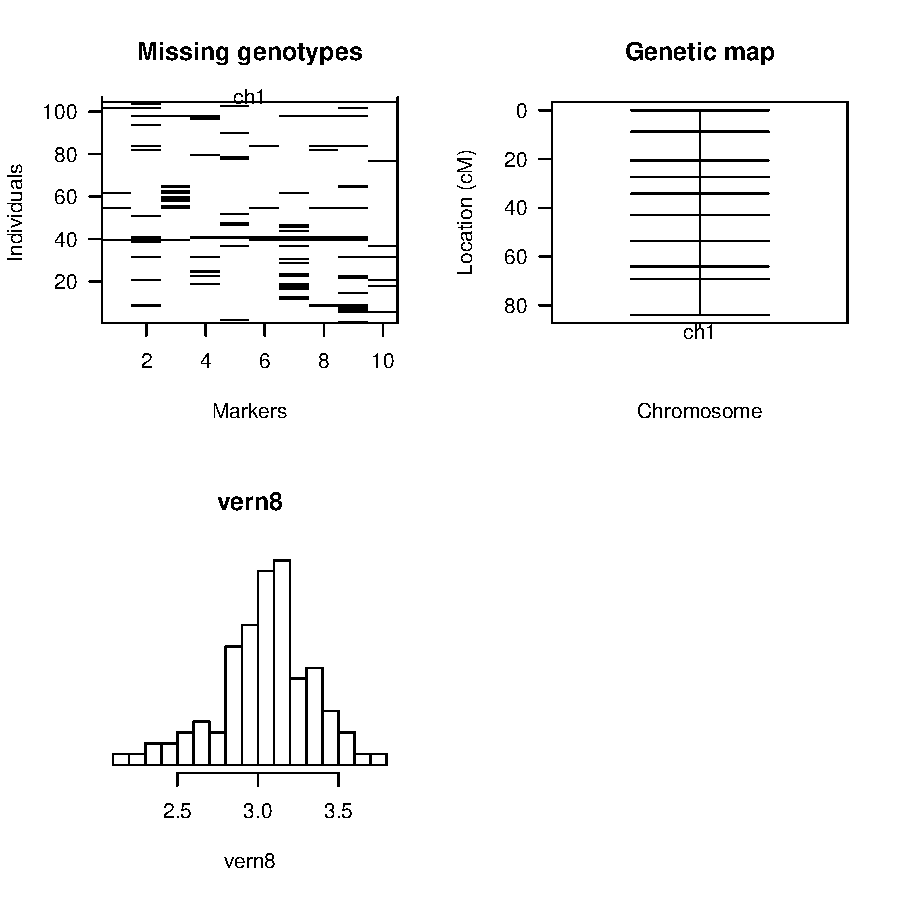
\includegraphics{bim_summary-002}

These data are treated as a backcross (although in fact they are from
a double haploid, homozygous at every locus). The plot, from library
R/qtl, shows the pattern of missing genotypes, the linkage map, and
the 11 traits. We focus on \texttt{log10flower8}, the logarithm base
10 of the flowering time after eight weeks of vernalization.

Bayesian interval mapping proceeds by first running the
\texttt{bmapqtl} Markov chain Monte Carlo simulation of the posterior.

\begin{Schunk}
\begin{Sinput}
> bmapqtl.options(prior.nqtl = "poisson")
\end{Sinput}
\begin{Soutput}
simulate 400000 MCMC steps, recording by 400 with 0.05 burnin and 0.05 pre-burnin
prior for number of QTL: poisson(3)
initial number of QTL: 0 
hyperparameters for priors:
             1  2
init       0.5 -1
prior.mean 1.0 -1
prior.var  3.0 -1
prior.add  0.0  0
prior.dom  0.0  0
random seed: 0 
\end{Soutput}
\end{Schunk}

\begin{Schunk}
\begin{Sinput}
> vernpois.bim = run.bmapqtl(vern)
\end{Sinput}
\begin{Soutput}
Bayesian interval mapping MCMC run in progress. 
Count of 1000 iterations shown separated by dots (negative for burnin):
-20.-15.-10.-5.0.
5.10.15.20.25.30.35.40.45.50.
55.60.65.70.75.80.85.90.95.100.
105.110.115.120.125.130.135.140.145.150.
155.160.165.170.175.180.185.190.195.200.
205.210.215.220.225.230.235.240.245.250.
255.260.265.270.275.280.285.290.295.300.
305.310.315.320.325.330.335.340.345.350.
355.360.365.370.375.380.385.390.395.
\end{Soutput}
\end{Schunk}

Now that we have the MCMC simulations, we can examine diagnostic
plots. First, time series of the burnin and MCMC runs gives a
graphical idea of how well the simulations are `mixing'.
 
\begin{Schunk}
\begin{Sinput}
> plot.bim.mcmc(vernpois.bim)
\end{Sinput}
\end{Schunk}
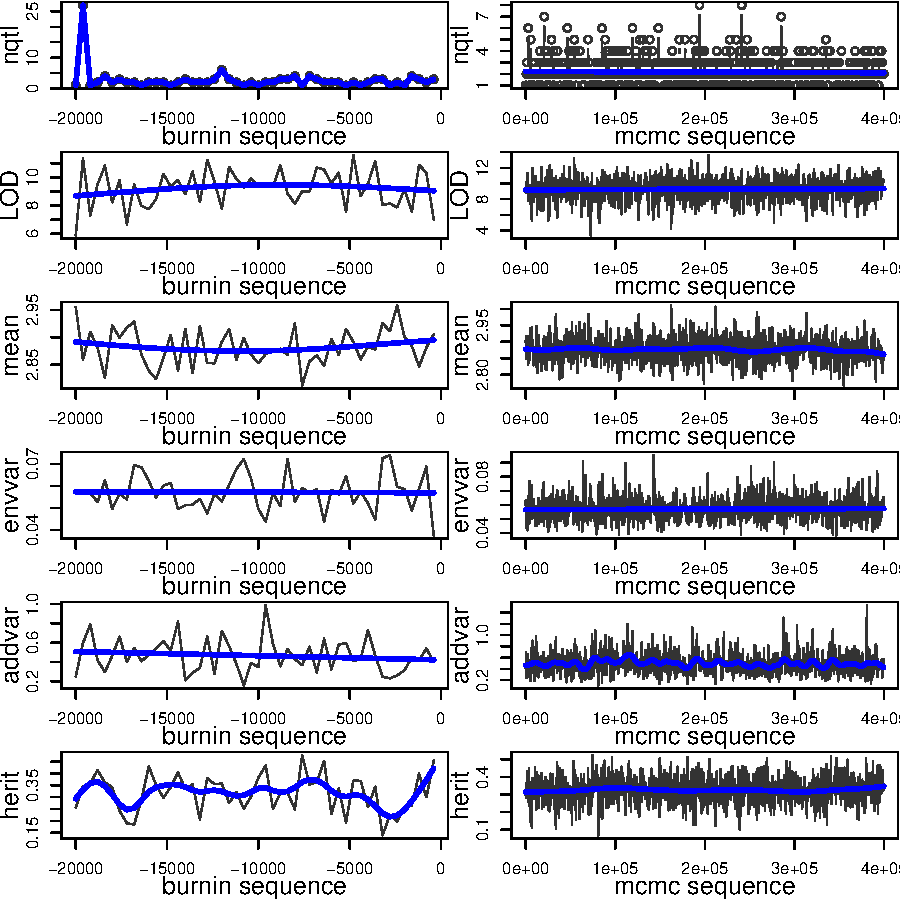
\includegraphics{bim_summary-005}

A jittered plot of quantitative trait loci by chromosome shows the
where the posterior concentrates along the genome relative to the
marker map.

\begin{Schunk}
\begin{Sinput}
> plot.bim.loci(vernpois.bim, vern)
\end{Sinput}
\end{Schunk}
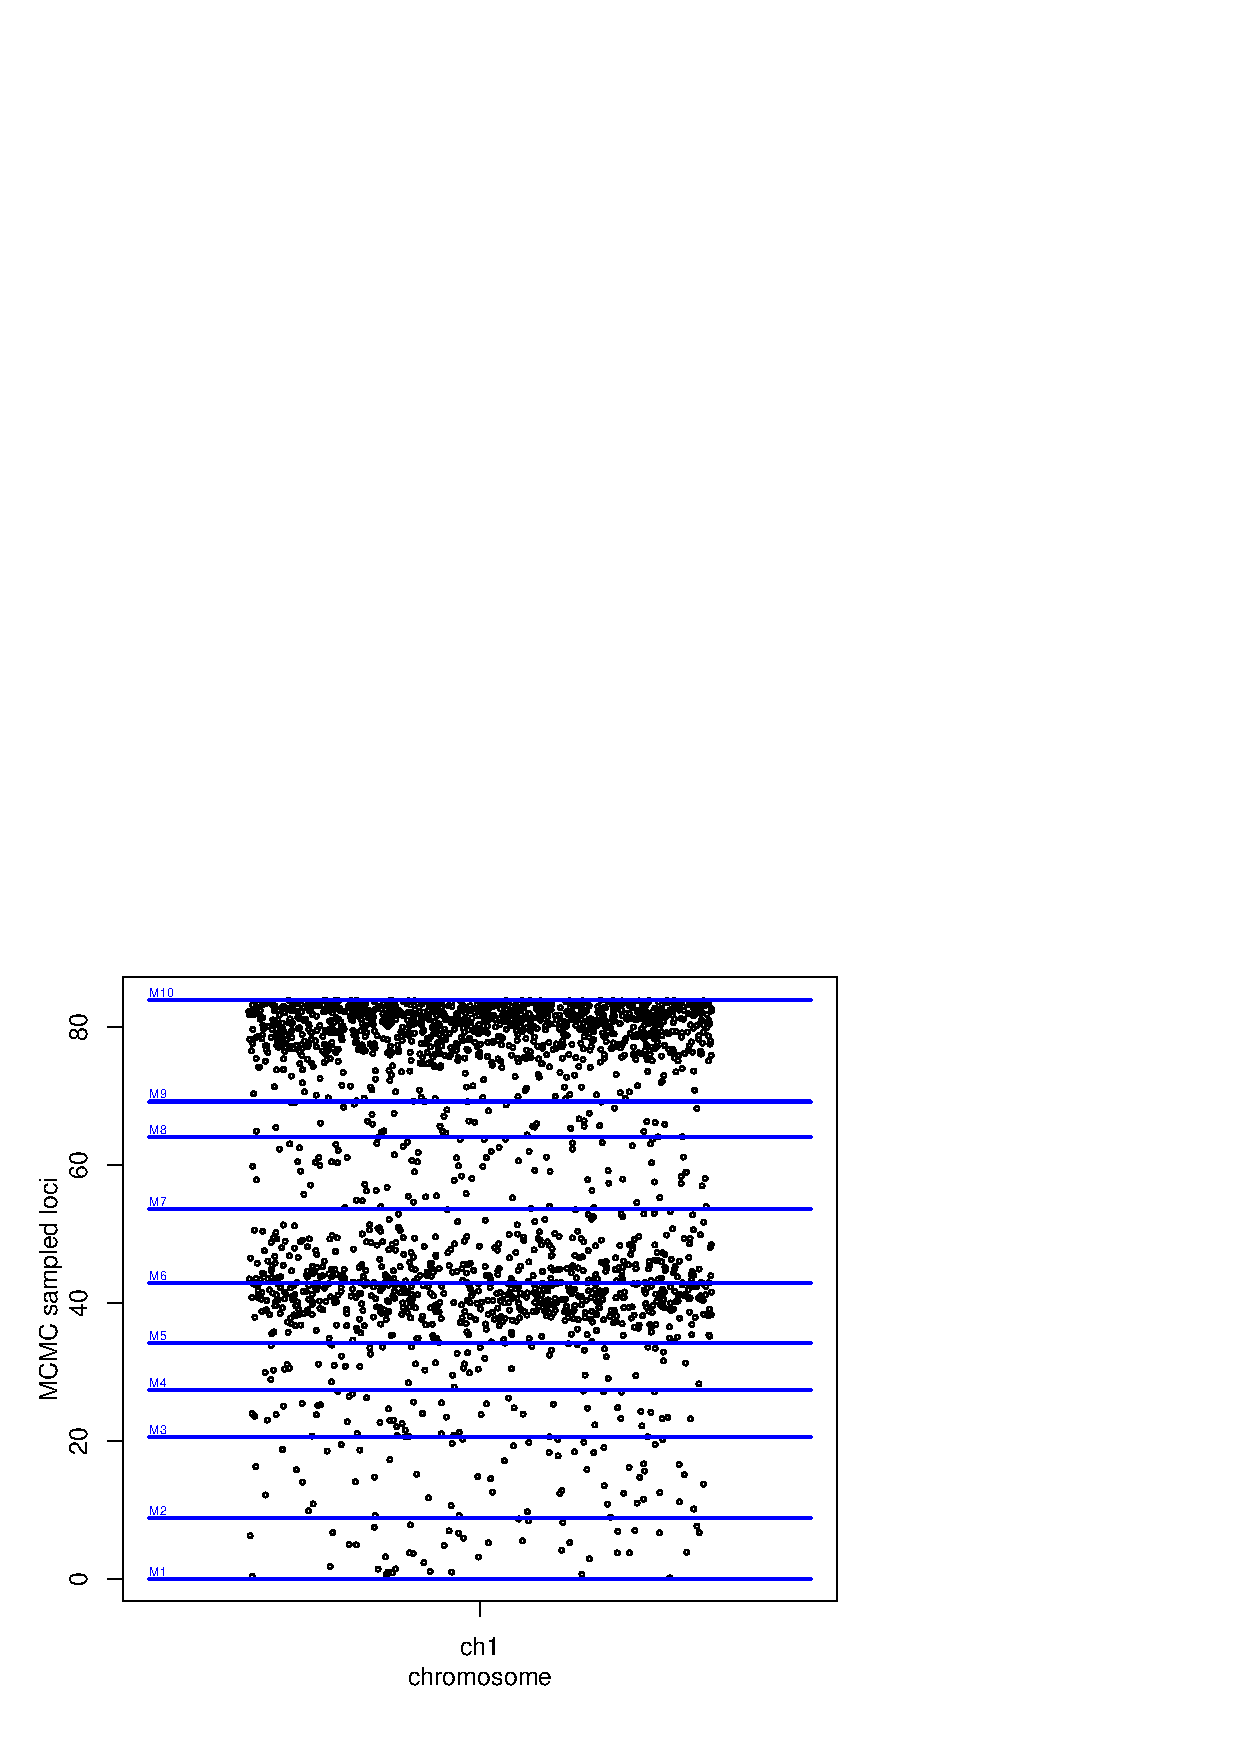
\includegraphics{bim_summary-006}

Model selection is assisted by four plots. The top two concern the
number of QTL while the bottom two are for the pattern of loci across
chromosomes. The left panel shows the posterior as a histogram,
overlaid by the prior (rescaled to fit). The right panel show the
posterior to prior ratios which make up Bayes factors. A large
vertical separation on a log scale indicates substantial difference
among models. The summary shows in numbers what is found in the plots.

\begin{Schunk}
\begin{Sinput}
> model = bim.model(vernpois.bim, vern)
> summary(model)
\end{Sinput}
\begin{Soutput}
posterior for number of QTL as %
 1  2  3  4  5  6  7  8 
22 52 17  6  2  0  0  0 
Bayes factor ratios for number of QTL
  1   2   3   4   5   6   7   8 
1.0 1.6 0.5 0.2 0.1 0.1 0.1 0.2 
model posterior above cutoff 1 as %
2*1   1 3*1 4*1 5*1 
 52  22  17   6   2 
Bayes factor ratios for chromosome pattern
2*1   1 3*1 4*1 5*1 
1.0 1.3 0.2 0.1 0.0 
\end{Soutput}
\begin{Sinput}
> plot(model)
\end{Sinput}
\begin{Soutput}
$nqtl
$nqtl$posterior

    1     2     3     4     5     6     7     8 
0.222 0.519 0.172 0.062 0.016 0.005 0.002 0.002 

$nqtl$prior
          1           2           3           4           5           6 
0.149361205 0.224041808 0.224041808 0.168031356 0.100818813 0.050409407 
          7           8 
0.021604031 0.008101512 

$nqtl$bf

         1          2          3          4          5          6          7 
1.00000000 1.55855856 0.51651652 0.24824825 0.10677344 0.06673340 0.06228451 
         8 
0.16609202 

$nqtl$bfse

         1          2          3          4          5          6          7 
0.05919886 0.04744735 0.03583729 0.03053457 0.02647895 0.02976938 0.04399773 
         8 
0.11732729 


$pattern
$pattern$posterior
  2*1     1   3*1   4*1   5*1 
0.519 0.222 0.172 0.062 0.016 

$pattern$prior
       2*1          1        3*1        4*1        5*1 
0.14936121 0.04978707 0.22404181 0.22404181 0.16803136 

$pattern$bf
       2*1          1        3*1        4*1        5*1 
1.00000000 1.28323699 0.22093770 0.07964033 0.02740313 

$pattern$bfse
        2*1           1         3*1         4*1         5*1 
0.030443099 0.075966162 0.015329245 0.009795772 0.006795754 


$param
$param$nqtl
[1] 1

$param$pattern
NULL

$param$exact
[1] FALSE

$param$cutoff
[1] 1


attr(,"class")
[1] "bim.model"
\end{Soutput}
\end{Schunk}
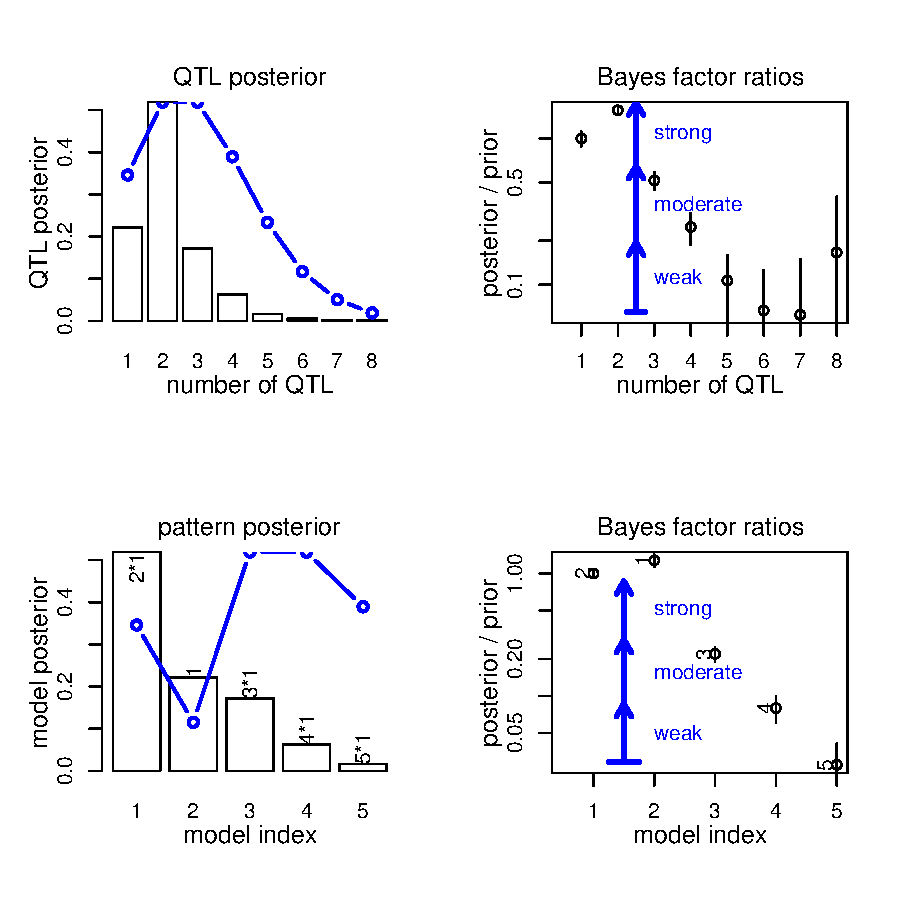
\includegraphics{bim_summary-007}

The effects plots show the quantitative trait loci by a histogram and
density (blue) on the top plot and effects (additive and possibly
dominance) in scatter plot with a smoothing spline fit plus or minus
two standard errors. Vertical lines (red) identify the estimated QTL.
The summary shows the estimated QTL loci and effects.

\begin{Schunk}
\begin{Sinput}
> qtl = plot.bim.effects(vernpois.bim, vern)
> summary(qtl)
\end{Sinput}
\begin{Soutput}
QTL loci and density peaks:
  chr     loci      dens
1 ch1 81.28166 0.0579028

HPD region density cutoffs:
        0.5        0.55         0.6        0.65         0.7        0.75 
0.027622297 0.025171976 0.022465807 0.019018241 0.015372926 0.011697632 
        0.8        0.85         0.9        0.95 
0.007841648 0.004631643 0.003782281 0.002930640 

QTL loci and effect estimates:
    chrom     loci       add     add.sd
ch1   ch1 81.28166 0.2217985 0.08198312
     mean       NA 2.8760781 0.03777311

QTL density estimates by chromosome at 512 grid points with bw = 2 

Smoothing spline parameters for additive effects:
      ch1 
0.9004665 
\end{Soutput}
\end{Schunk}
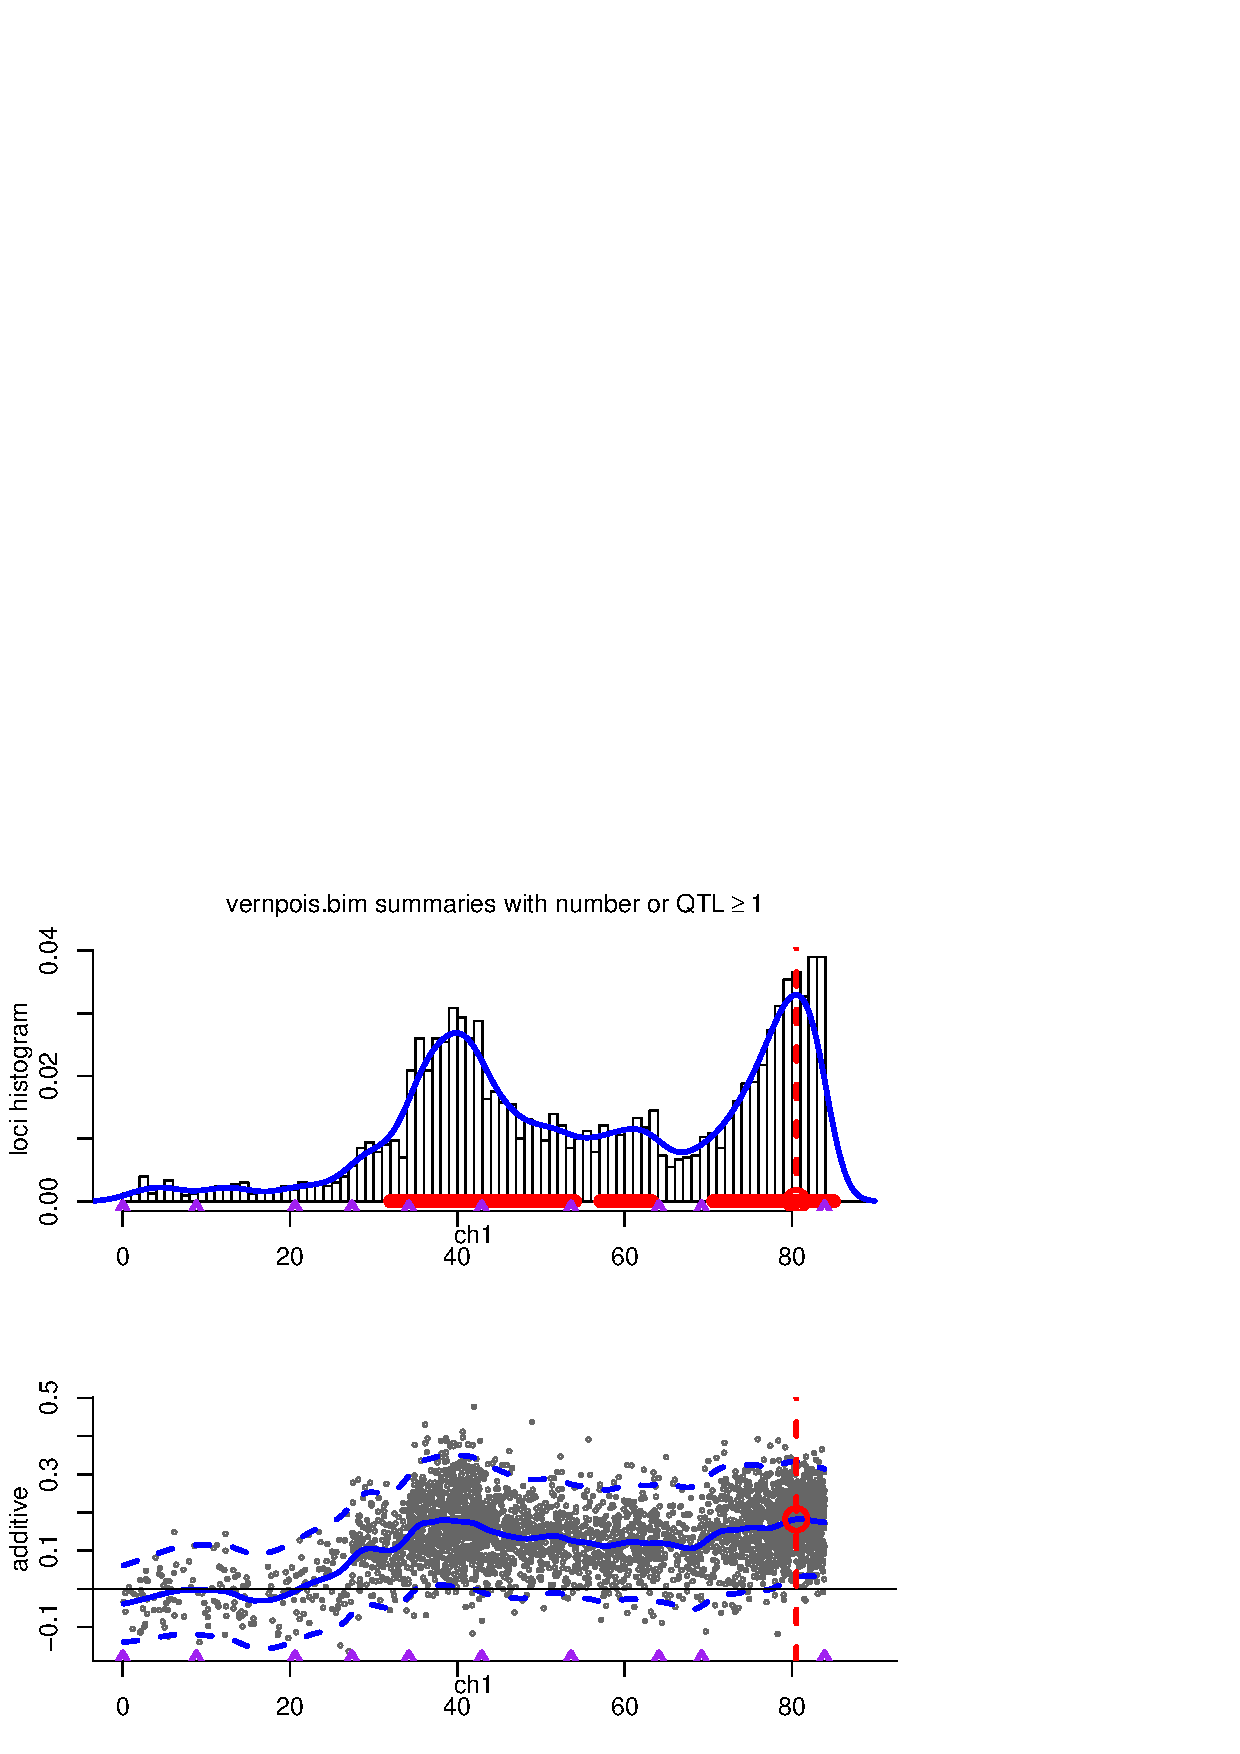
\includegraphics{bim_summary-008}

Finally, summary diagnostics for model parameters are shown as
histograms and boxplots conditional on the number of QTL. Notice how
the boxplots level out as the model gets more complex, although there
is very little data for models with a large number of QTL.

\begin{Schunk}
\begin{Sinput}
> plot.bim.diag(vernpois.bim)
\end{Sinput}
\begin{Soutput}
LOD 9.372 
conditional LOD 
     1      2      3      4      5      6      7      8 
 7.978  9.633  9.771  9.971  9.699  9.961  9.096 11.138 
mean 2.876 
conditional mean 
    1     2     3     4     5     6     7     8 
2.896 2.869 2.873 2.871 2.884 2.870 2.915 2.905 
envvar 0.056 
conditional envvar 
    1     2     3     4     5     6     7     8 
0.058 0.056 0.055 0.054 0.055 0.061 0.055 0.047 
addvar 0.473 
conditional addvar 
    1     2     3     4     5     6     7     8 
0.423 0.475 0.481 0.520 0.429 0.642 0.302 0.590 
herit 0.326 
conditional heritability 
    1     2     3     4     5     6     7     8 
0.296 0.331 0.331 0.343 0.316 0.306 0.291 0.341 
\end{Soutput}
\end{Schunk}
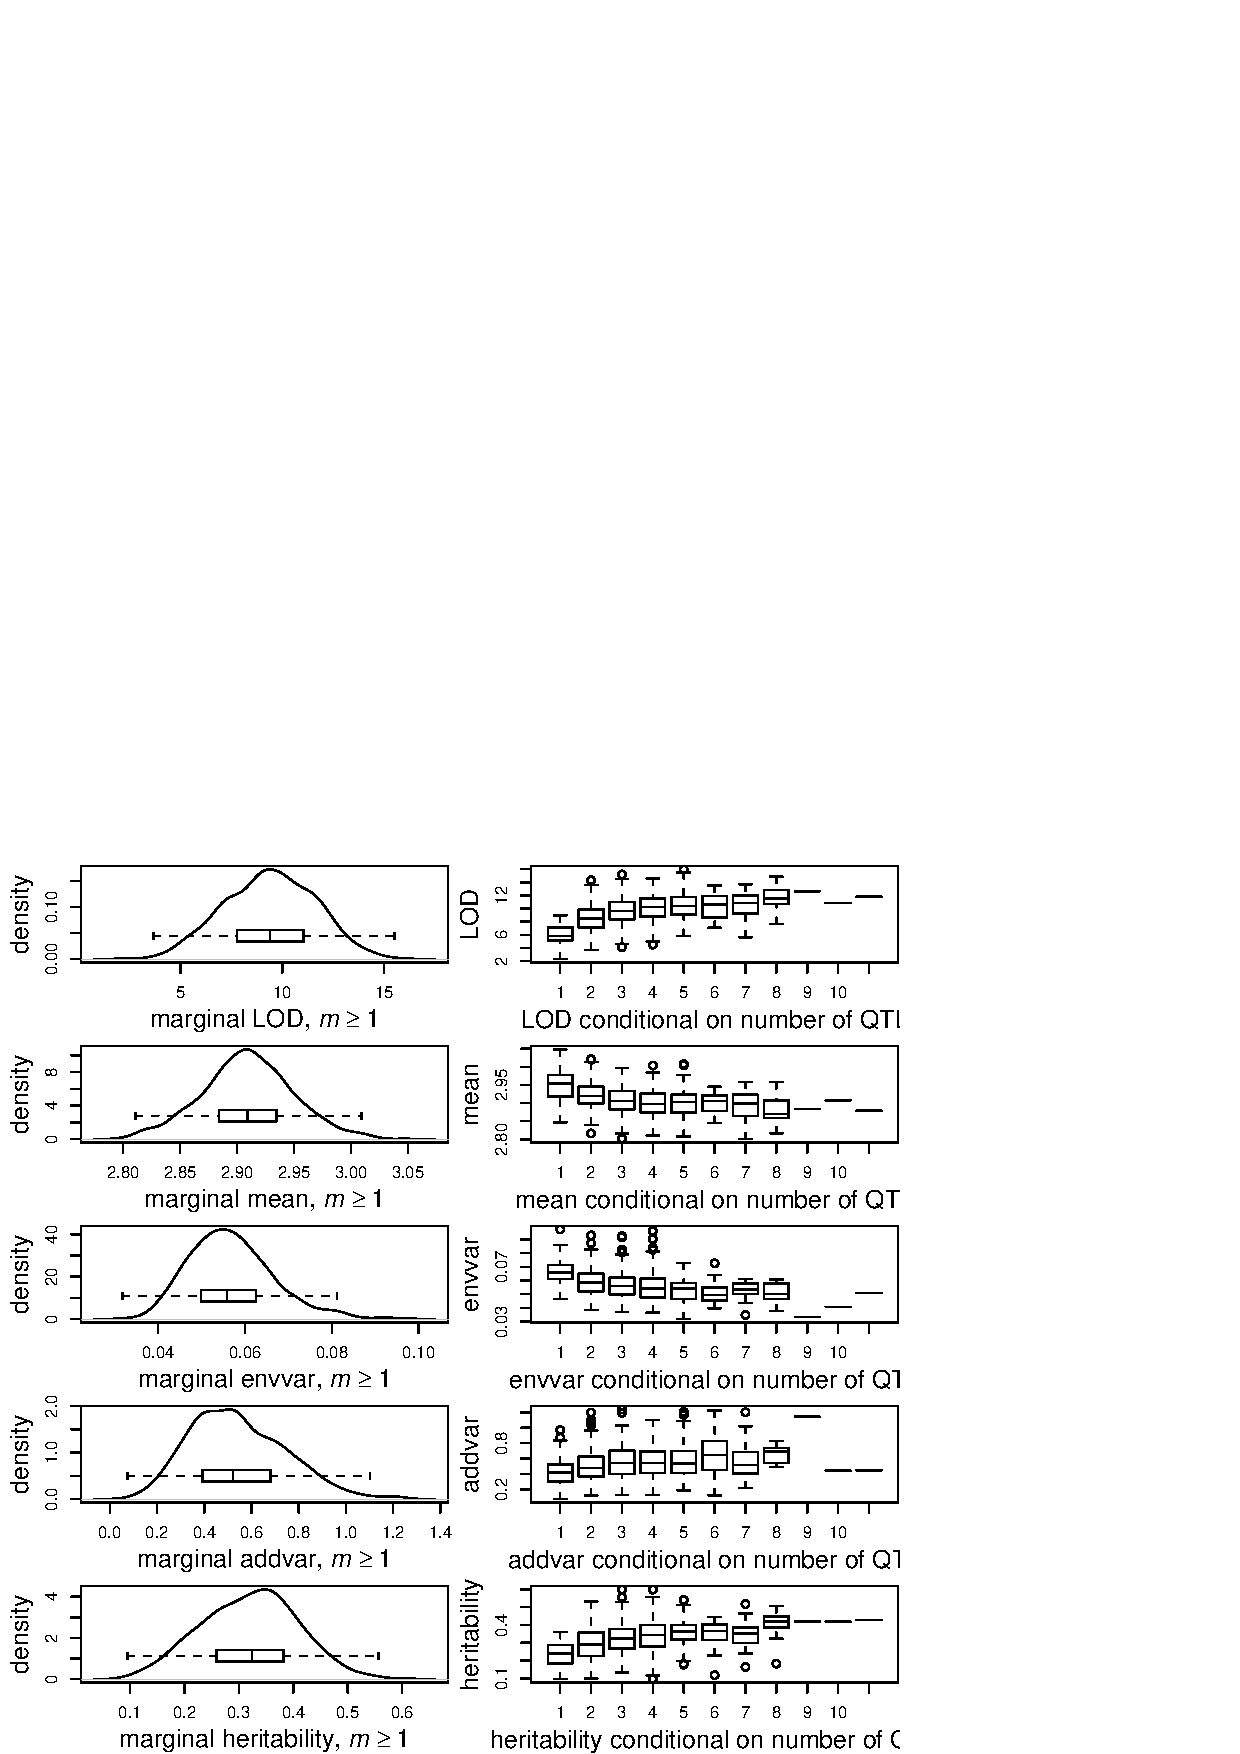
\includegraphics{bim_summary-009}

All of these plots can be produced by one call to
\texttt{plot(vernpois.bim,vern)}. Following this intial investigation, we
can refine our graphics by restricting attention to `better'
models. For instance, the model selection suggests two QTL on the
chromosome. The option \texttt{pattern}  can pick up only those
simulations that have 2 QTL on this chromosome. We can then reexamine
the model

\begin{Schunk}
\begin{Sinput}
> plot.bim.model(vernpois.bim, vern, pattern = c(1, 1))
\end{Sinput}
\begin{Soutput}
$nqtl
$nqtl$posterior

          2           3           4           5           6           7 
0.667095116 0.221079692 0.079691517 0.020565553 0.006426735 0.002570694 
          8 
0.002570694 

$nqtl$prior
          2           3           4           5           6           7 
0.224041808 0.224041808 0.168031356 0.100818813 0.050409407 0.021604031 
          8 
0.008101512 

$nqtl$bf

         2          3          4          5          6          7          8 
1.00000000 0.33140655 0.15928067 0.06850781 0.04281738 0.03996289 0.10656771 

$nqtl$bfse

         2          3          4          5          6          7          8 
0.02532657 0.02230198 0.01940591 0.01694993 0.01908689 0.02822169 0.07525783 


$pattern
$pattern$posterior
       2*1        3*1        4*1        5*1 
0.66709512 0.22107969 0.07969152 0.02056555 

$pattern$prior
      2*1       3*1       4*1       5*1 
0.1493612 0.2240418 0.2240418 0.1680314 

$pattern$bf
       2*1        3*1        4*1        5*1 
1.00000000 0.22093770 0.07964033 0.02740313 

$pattern$bfse
        2*1         3*1         4*1         5*1 
0.025326572 0.014867985 0.009702953 0.006779970 


$param
$param$nqtl
[1] 1

$param$pattern
[1] 1 1

$param$exact
[1] FALSE

$param$cutoff
[1] 1


attr(,"class")
[1] "bim.model"
\end{Soutput}
\end{Schunk}
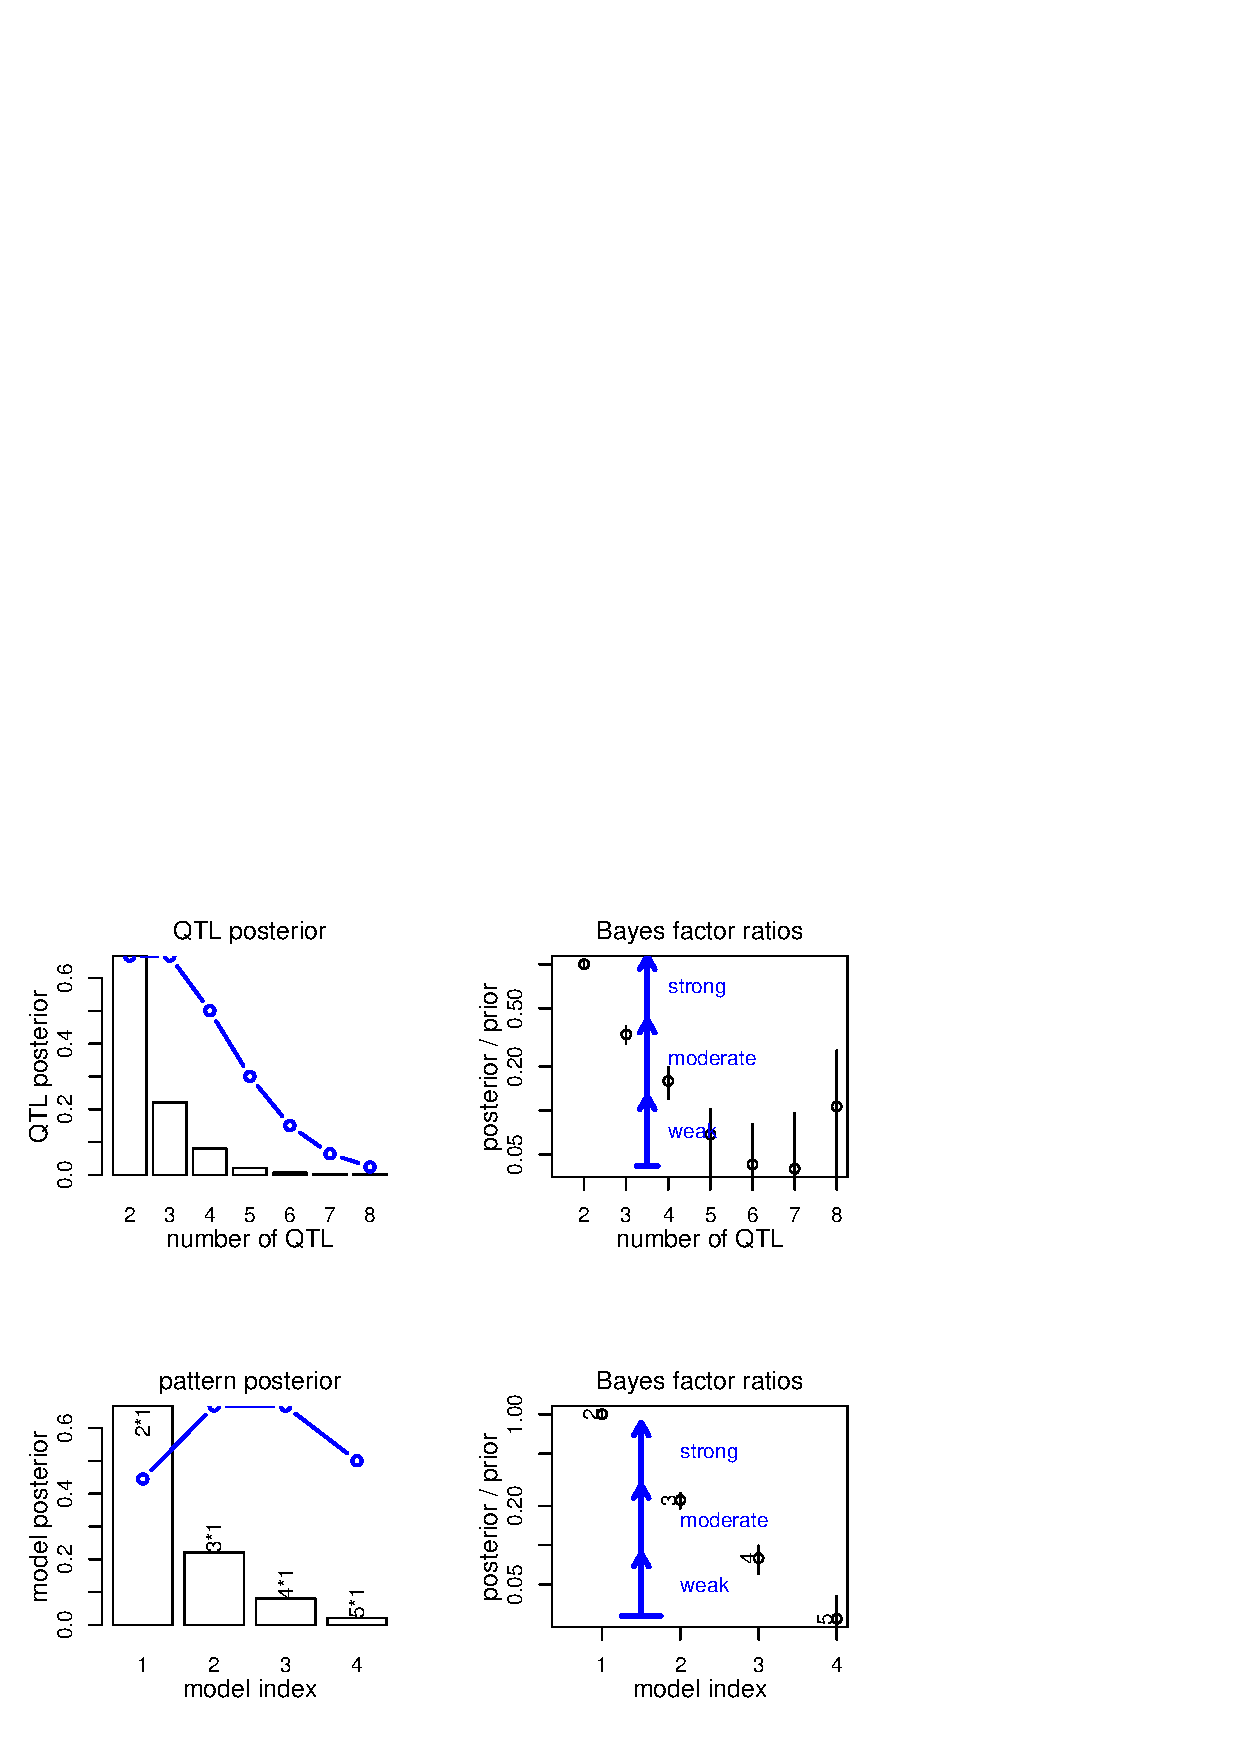
\includegraphics{bim_summary-010}

\noindent and reexamine the effects

\begin{Schunk}
\begin{Sinput}
> plot.bim.effects(vernpois.bim, vern, pattern = c(1, 1))
\end{Sinput}
\end{Schunk}
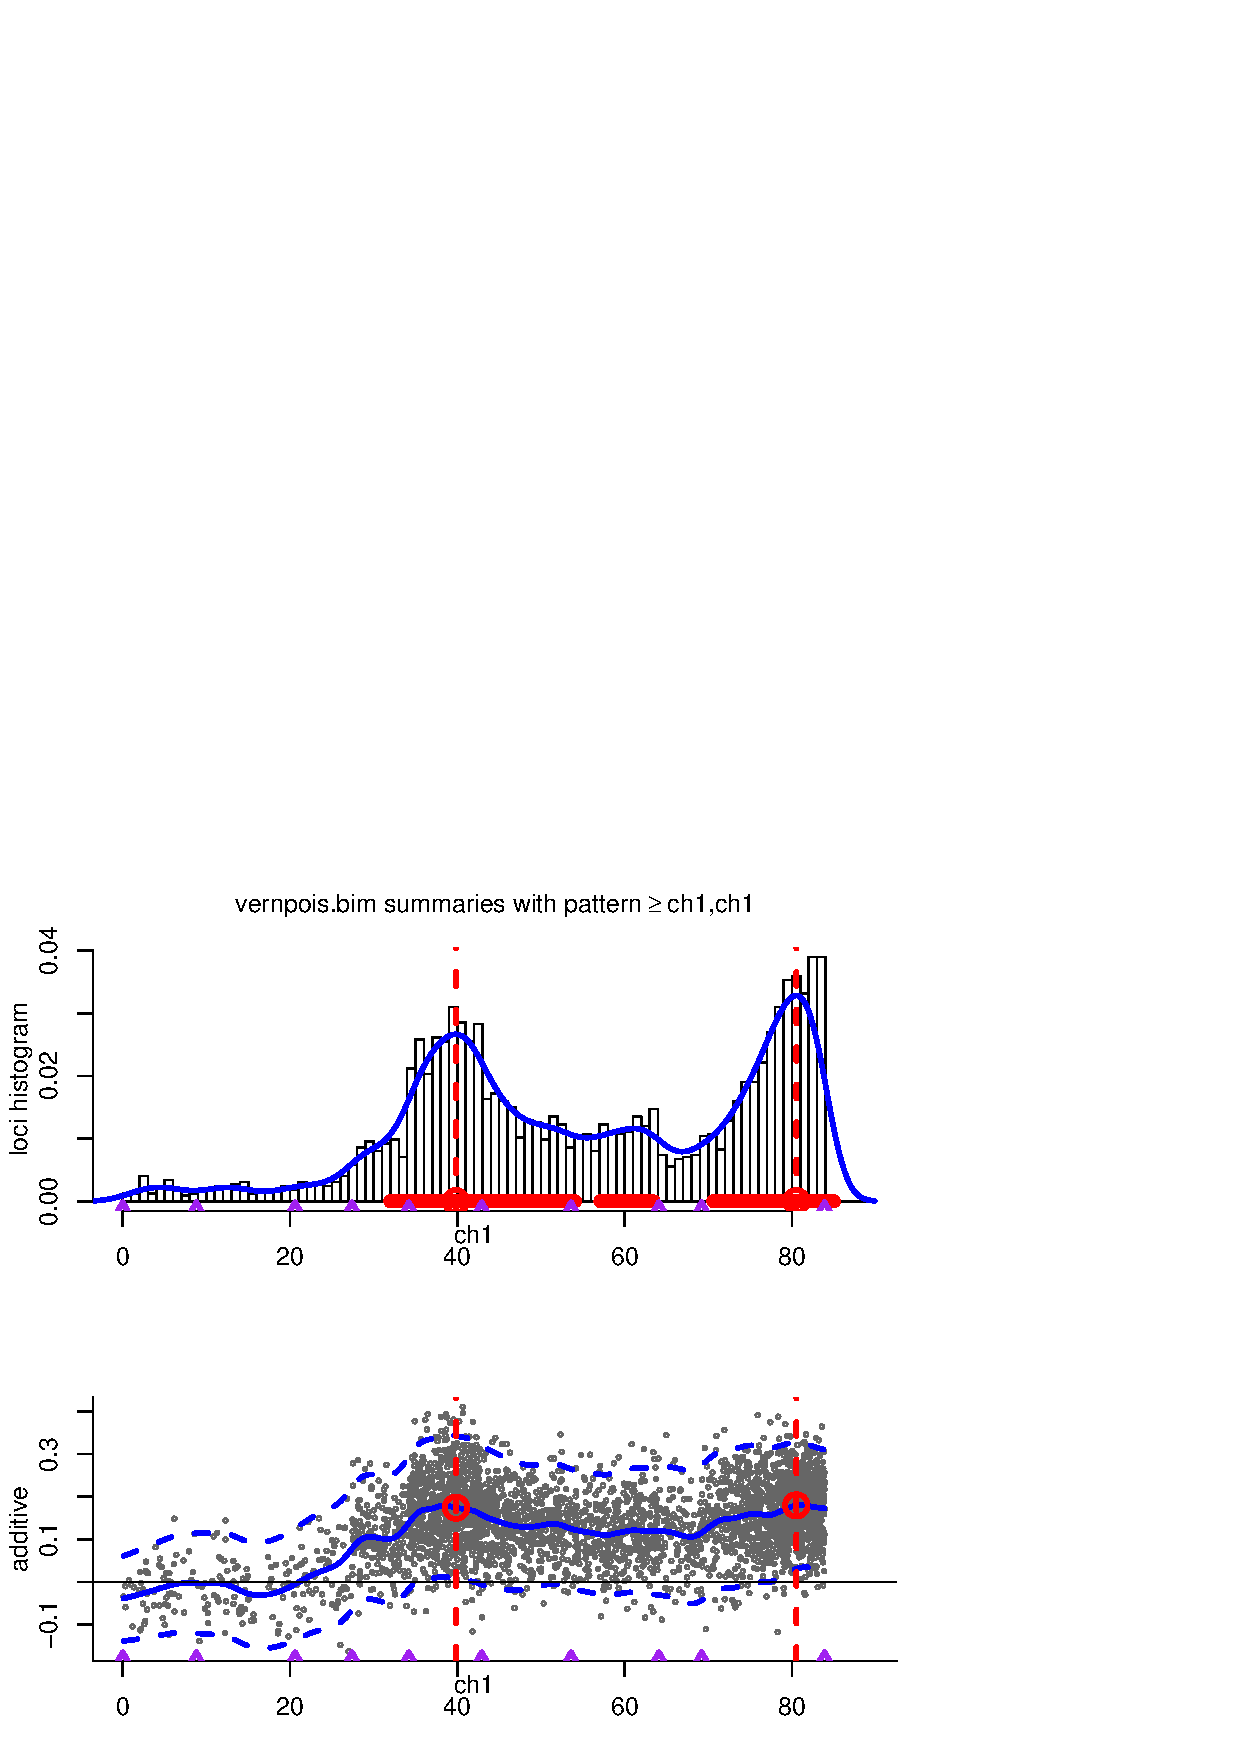
\includegraphics{bim_summary-011}

\noindent This subsetting is even more effective for full-genome
studies. Consider analyzing the full \texttt{Bnapus} dataset for the
trait \texttt{log10flower8}.

We can assess the false discovery rate, which gives us some feedback
on the width of highest probability density (HPD) regions for QTLs
(horizontal red lines on loci histograms).

\begin{Schunk}
\begin{Sinput}
> plot.bim.fdr(vernpois.bim, vern, pattern = c(1, 1))
\end{Sinput}
\begin{Soutput}
       H0        M0        M1 
0.2353702 0.0000000 1.0000000 
$hyp
   H0    M0    M1 
0.235 0.000 1.000 

$fdr
0.05  0.1 0.15  0.2 0.25 
0.19 0.74 0.87 0.95 0.99 
\end{Soutput}
\end{Schunk}
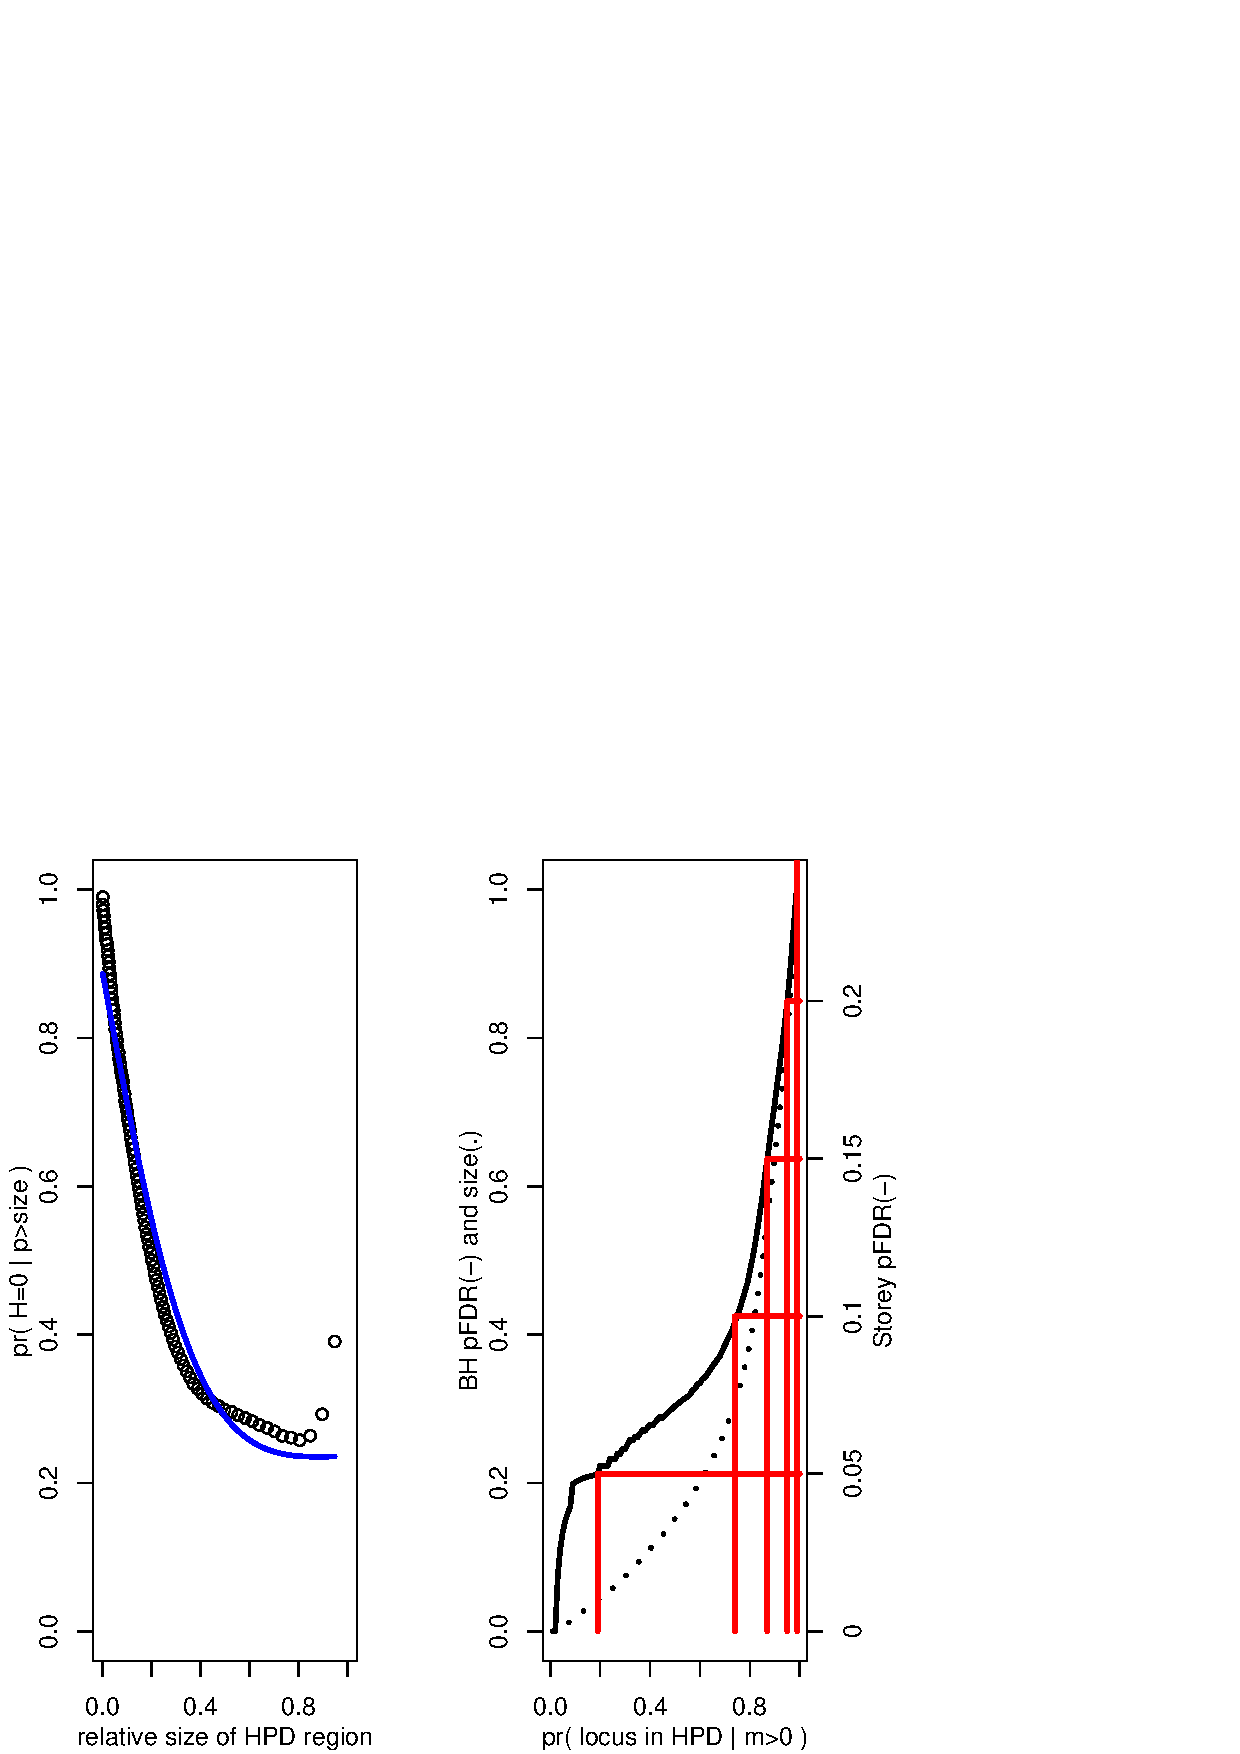
\includegraphics{bim_summary-012}

\end{document}
